\chapter{Introduction}

Cities are a central feature of human society - Human beings are increasingly an urban species. Cities are one of the primary sources of technological development and increasing wealth. Behind these observations is a fundamental feature demonstrated in the recent literature on scaling laws: the productivity of cities increases super-linearly in population. Cities are the locus of a positive feedback loop: rising populations raises productivity, rising productivity attracts more people and resource.

Cities are where people live and work, where a great deal of production is concentrated, in addition to being where wealth is created and accumulated, cities are also where income is actually distributed. 

In Canada, there is a housing crisis. In the last few years, the need for affordable housing has come into focus as one of the most pressing issues facing Canadians. As more and more Canadians are finding housing unaffordable, the effects are being seen in everything from declining home ownership rates to an increasing number of Canadians unable to afford housing at all.

There has been extensive work on the drivers of the crisis, including supply shortages, stagnating incomes, and the finacialization of housing ownership.

There has been less work on the implications for productivity. The housing crisis raises the question of whether Canadian cities can continue to attract people and accumulate wealth for its residents and industries, whether in fact it can even sustain their growth.

This thesis presents a spatial model of the city that incorporates distributional issues and financialization and allows us to examine the productivity implications of the housing crisis. The model that incorporates the scaling of productivity in cities within a standard urban model. 
The urban model is based on those developed in geography, planning and urban economics. The organizing principle in  the spatial models of all three disciplines is an economic variable, land rent, which is the link to distribution, financialization and continuing productivity. *** (another sentence on why this is great)

The analysis makes clear that in addition to the recognized distributional consequences, the housing crisis has productivity impacts that should be considered in developing urban and housing policy. Sopecifically, the analysis in this thesis concludes that, given the ongoing financialization of the housing market,


\begin{enumerate}
\item the financial system will eventually extract all net urban land rents through investment in urban property
\item housing accessibility will become increasingly challenging for disadvantaged groups
\item housing will be largely eliminated as a saving mechanism and asset fr middle income Canadians,  resulting in a systematic decline in the `middle class'
\item that the quality of urban life will decline
\item the economic growth and development of cities is threatened by this financialization
\end{enumerate}


The focus of this thesis on a topic. that falls in the overlap  between least three academic  disciplines, Economics, Urban Geography, and Planning. The central and shared concern in this area is with geographic space.



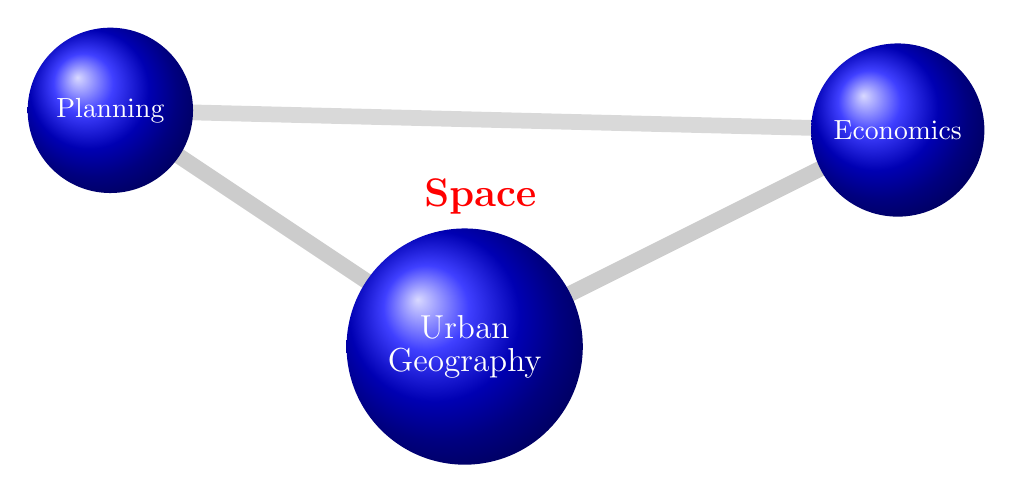
\begin{tikzpicture}{scale=.5}
% find color cotrol for ball. Tind way to stop line short of node
\coordinate (planning) at (-5,1);%PREFACE
\coordinate (economics) at (5,.75);%
 \coordinate (geography) at (-.5,-2); %history
\coordinate (finance) at (0,5); %

\draw [line width=2mm, black!15, ] (planning)--(economics);
\draw [line width=2mm, black!20, ] (geography)--(economics);
\draw [line width=2mm, black!20, ] (geography)--(planning);

%\draw [line width=2mm, black!25, ] (geography)--(finance);
%\draw [line width=2mm, black!20, ] (planning)--(finance);
%\draw [line width=2mm, black!20, ] (finance)--(economics);

\node [circle,shading=ball, minimum width=2.1   cm, white, align=center] (ball) at (planning) {Planning};
\node [circle,shading=ball, minimum width=2.2cm, white, align=center] (ball) at (economics) {Economics};
\node [circle,shading=ball, minimum width=3 . cm, white, align=center] (ball) at (geography)[text width=2cm] {\large Urban\\ Geography};

%\node [circle, shading=ball, minimum width=2.4cm, white, align=center] (ball) at (finance)[text width=2cm] {Finance};

\node at (-.3,-.1) [red] {\Large \textbf{Space}};
\end{tikzpicture}

Figure 1: The common concern of three fields
topic 

A simple economic insight -- that locational value gives rise to land rents -- provides an organizing principle for the three disciplines. Rent theory has a long history in economics, going back to thinkers such as Richard Cantillon (1680s-1734), François Quesnay (1694–1774), the marquis de Mirabeau (1715–1789) and Anne-Robert-Jacques Turgot (name physiocrat) and Adam Smith (1723-1790) and received its classic statement in Ricardo (1772-1823). Nearly contemporaneous thinker, Johann Heinrich  von Th\"unen (1783-1850) developed a planning model to guide the location of economic activities for an urban-agricultural society.  A version of that model  was reinvented in urban geography by XXX. Alonzo\footnote{We use a version of the well-established model of Alonso (1964), Muth (1969) and Mills (1967), and formalised by Wheaton (1974),}

We link the Alonzo model with more recent work on growth theory starting with Robert Solo's XXX and with the endogenous growth models of Lucas () and draw on Jane Jacobs's insight that endogenous urban growth  is. now driving economic development. Jacobs's insight is empirically supported by recent work in the complexity literature on urban scaling by XXXX ()




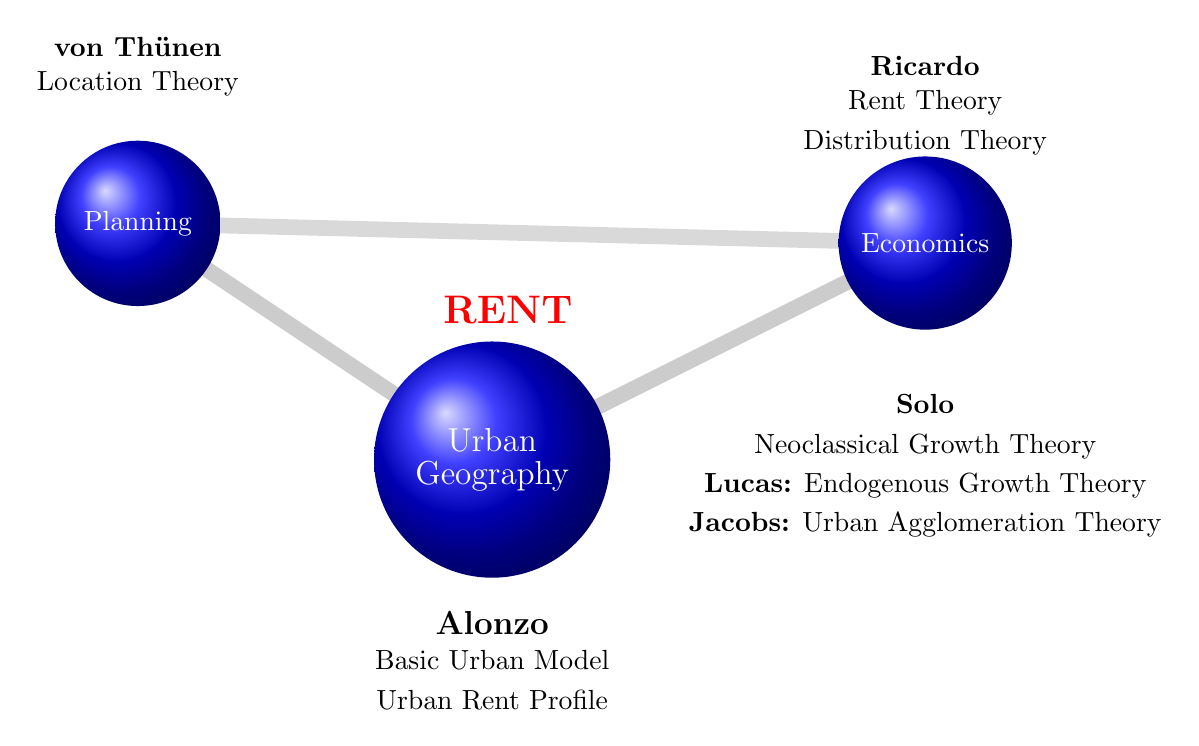
\begin{tikzpicture}{scale=.5}
% find color cotrol for ball. Tind way to stop line short of node
\coordinate (planning) at (-5,1);%PREFACE
\coordinate (economics) at (5,.75);%
 \coordinate (geography) at (-.5,-2); %history
\coordinate (finance) at (0,5); %

\draw [line width=2mm, black!15, ] (planning)--(economics);
\draw [line width=2mm, black!20, ] (geography)--(economics);
\draw [line width=2mm, black!20, ] (geography)--(planning);

%\draw [line width=2mm, black!25, ] (geography)--(finance);
%\draw [line width=2mm, black!20, ] (planning)--(finance);
%\draw [line width=2mm, black!20, ] (finance)--(economics);

\node [circle,shading=ball, minimum width=2.1   cm, white, align=center] (ball) at (planning) {Planning};
\node [circle,shading=ball, minimum width=2.2cm, white, align=center] (ball) at (economics) {Economics};
\node [circle,shading=ball, minimum width=3 . cm, white, align=center] (ball) at (geography)[text width=2cm] {\large Urban\\ Geography};

%\node [circle, shading=ball, minimum width=2.4cm, white, align=center] (ball) at (finance)[text width=2cm] {Finance};

\node at (-.3,-.1) [red] {\Large \textbf{RENT}};

% new stuff
\node at (planning) [above=2cm] {\textbf{von Th\"unen}};
\node at (planning) [above=1.5cm] {Location Theory};

\node at (economics) [above=2cm] {\textbf{Ricardo}};
\node at (economics) [above=1.5cm] {Rent Theory};
\node at (economics) [above=1.0cm] {Distribution Theory};

\node at (economics) [below=1.8cm] {\textbf{Solo}};
\node at (economics) [below=2.3cm] {Neoclassical Growth Theory};
\node at (economics) [below=2.8cm] {\textbf{Lucas:} Endogenous Growth Theory};
\node at (economics) [below=3.3cm] {\textbf{Jacobs:} Urban Agglomeration Theory};


\node at (geography) [below=1.8cm] {\textbf{\large Alonzo}};
\node at (geography) [below=2.3cm] {Basic Urban Model};
\node at (geography) [below=2.8cm] {Urban Rent Profile};
\end{tikzpicture}

Figure 3: space and value

Land rent was historically the basis of the wealth and political power of  the land-owning class in the era of the classical economists.


We further link the model of urban rents to emerging concerns about the financialization of the housing market. The key insight we offer is that the financialization  of the housing sector is a  form of rent-seeking that must have detrimental effects on urban development and on the well-being of urban residents.





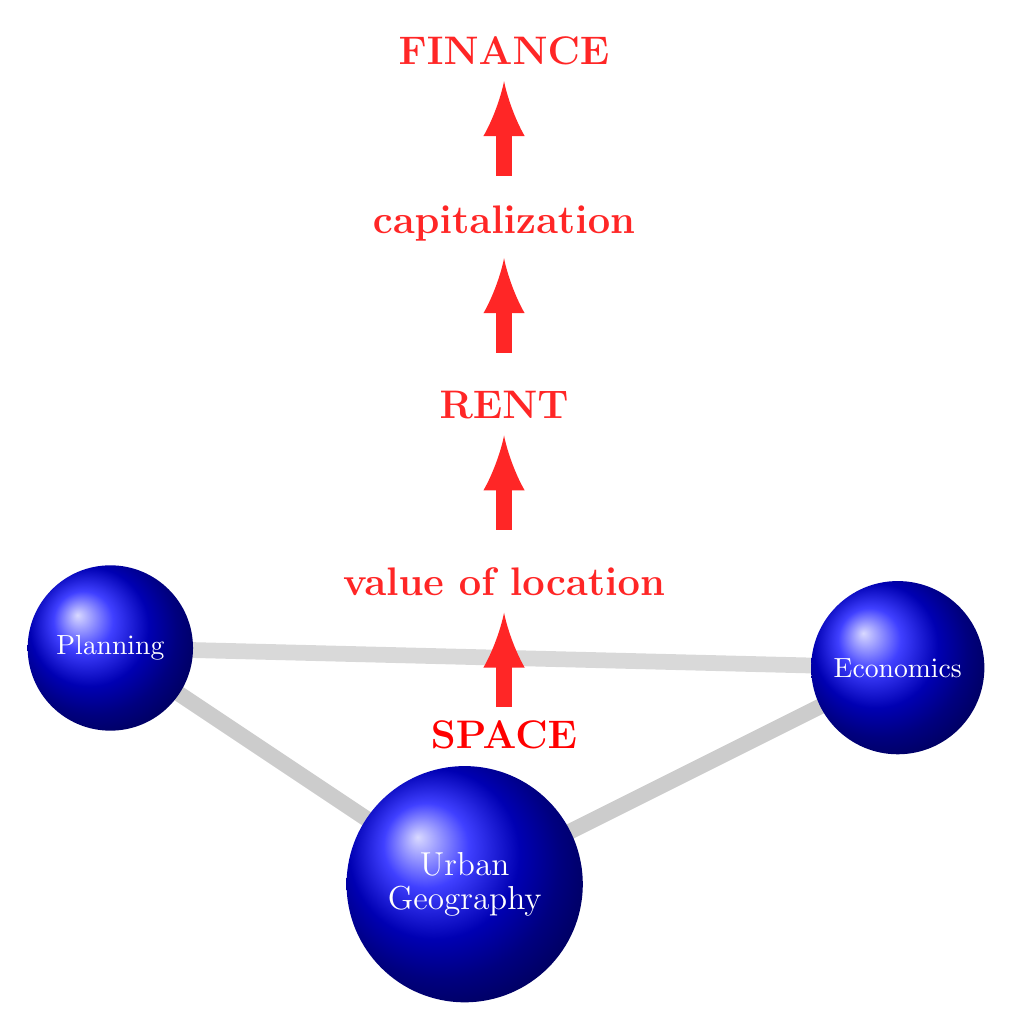
\begin{tikzpicture}{scale=.5}
% find color cotrol for ball. Tind way to stop line short of node
\coordinate (planning) at (-5,1);%PREFACE
\coordinate (economics) at (5,.75);%
 \coordinate (geography) at (-.5,-2); %history
\coordinate (finance) at (0,5); %

\draw [line width=2mm, black!15, ] (planning)--(economics);
\draw [line width=2mm, black!20, ] (geography)--(economics);
\draw [line width=2mm, black!20, ] (geography)--(planning);

%\draw [line width=2mm, black!25, ] (geography)--(finance);
%\draw [line width=2mm, black!20, ] (planning)--(finance);
%\draw [line width=2mm, black!20, ] (finance)--(economics);

\node [circle,shading=ball, minimum width=2.1   cm, white, align=center] (ball) at (planning) {Planning};
\node [circle,shading=ball, minimum width=2.2cm, white, align=center] (ball) at (economics) {Economics};
\node [circle,shading=ball, minimum width=3 . cm, white, align=center] (ball) at (geography)[text width=2cm] {\large Urban\\ Geography};

%\node [circle, shading=ball, minimum width=2.4cm, white, align=center] (ball) at (finance)[text width=2cm] {Finance};
\draw [line width=2mm, red!85, -latex ] (0, 7)--++(0,1.2)node[above=-.1] {\Large \textbf{FINANCE}};
\draw [line width=2mm, red!85, -latex ] (0, 4.75)--++(0,1.2)node[above=-.1] {\Large \textbf{capitalization}};
\draw [line width=2mm, red!85, -latex ] (0, 2.5)--++(0,1.2)node[above=-.1] {\Large \textbf{RENT}};
\draw [line width=2mm, red!85, -latex ] (0, .25)--++(0,1.2)node[above=-.1] {\Large \textbf{value of location}};
\node at (0,-.1) [red] {\Large \textbf{SPACE}};
\end{tikzpicture}



% \vspace {2cm}
% Figure 4 with finance

% \begin{tikzpicture}{scale=.5}
% % find color cotrol for ball. Tind way to stop line short of node
% \coordinate (planning) at (-5,1);%PREFACE
% \coordinate (economics) at (5,.75);%
%  \coordinate (geography) at (-.5,-2); %history
% \coordinate (finance) at (0,5); %

% \draw [line width=2mm, black!15, ] (planning)--(economics);
% \draw [line width=2mm, black!20, ] (geography)--(economics);
% \draw [line width=2mm, black!20, ] (geography)--(planning);

% \node at (-.3,2) [red] {\huge \textbf{RENT}};

% \draw [line width=3mm,  black!50,opacity=.5 ] (geography)--(finance);
% \draw [line width=2mm, black!20, ] (planning)--(finance);
% \draw [line width=2mm, black!20, ] (finance)--(economics);

% \node [circle,shading=ball, minimum width=2.1   cm, white, align=center] (ball) at (planning) {Planning};
% \node [circle,shading=ball, minimum width=2.2cm, white, align=center] (ball) at (economics) {Economics};
% \node [circle,shading=ball, minimum width=3 . cm, white, align=center] (ball) at (geography)[text width=2cm] {\large Urban\\ Geography};

% \node [circle, shading=ball, minimum width=2.4cm, white, align=center] (ball) at (finance)[text width=2cm] {Finance};


% \end{tikzpicture}

Summarizing the overall focus of the thesis,  we are concerned with the implication for urban development of growing rent extraction by the financial sector.  

\vspace {2cm}
Figure 4 with finance

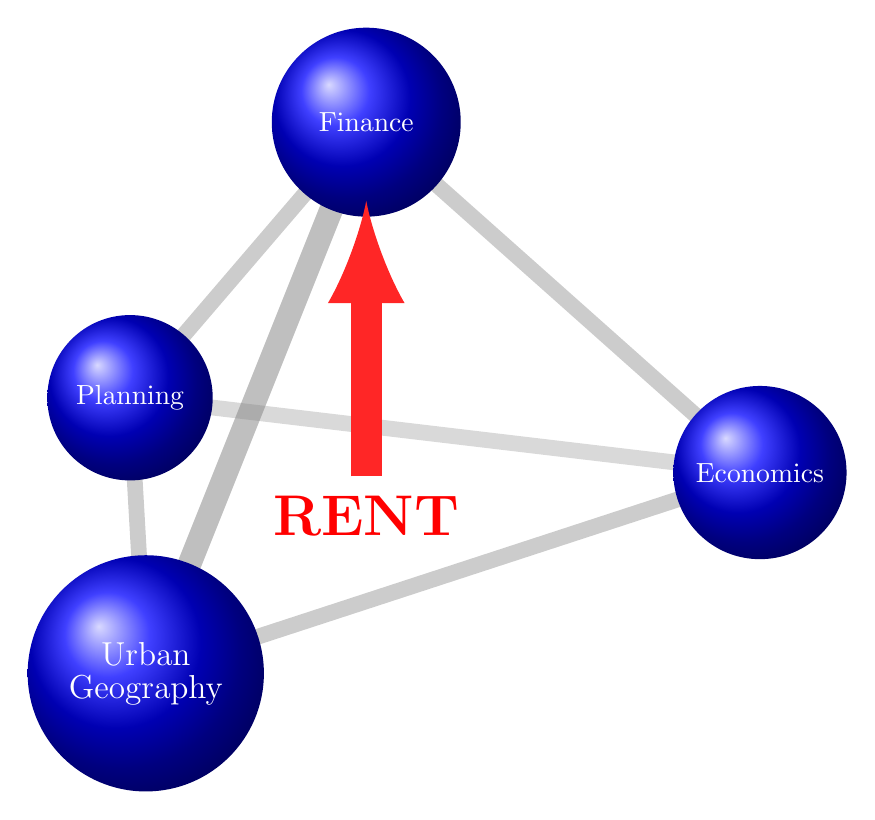
\begin{tikzpicture}{scale=.5}
% find color cotrol for ball. Tind way to stop line short of node
\coordinate (planning) at (-3,1.5);%PREFACE
\coordinate (economics) at (5,.55);%
 \coordinate (geography) at (-2.8,-2); %history
\coordinate (finance) at (0,5); %

\draw [line width=2mm, black!15, ] (planning)--(economics);
\draw [line width=2mm, black!20, ] (geography)--(economics);
\draw [line width=2mm, black!20, ] (geography)--(planning);

\node at (.0,0) [red] {\huge \textbf{RENT}};

\draw [line width=3mm,  black!50,opacity=.5 ] (geography)--(finance);
\draw [line width=2mm, black!20, ] (planning)--(finance);
\draw [line width=2mm, black!20, ] (finance)--(economics);

\node [circle,shading=ball, minimum width=2.1   cm, white, align=center] (ball) at (planning) {Planning};
\node [circle,shading=ball, minimum width=2.2cm, white, align=center] (ball) at (economics) {Economics};
\node [circle,shading=ball, minimum width=3 . cm, white, align=center] (ball) at (geography)[text width=2cm] {\large Urban\\ Geography};

\node [circle, shading=ball, minimum width=2.4cm, white, align=center] (ball) at (finance)[text width=2cm] {Finance};
\draw [line width=4mm, red!85, -latex ] (0, .5)--(0,4);


\end{tikzpicture}




\section{OVERVIEW OF DOCUMENT}
\color{blue}

\textbf{In chapter XXX}  we link classical rent theory, neoclassical production theory, neoclassical growth theory, the scaling literature, and urban spatial models.
To show how our model is directly connected with this broad collection of linked theories, we use the Cobb-Douglas function, which is used across this entire range of literature 

After we develop the mathematical description of the relationship among these will discuss  in more detail, rent theory and our contribution, scaling laws, ......  and other issues in the literature that draw on parts of this model and 

???  apply to the specific situation we're in why rent theory is related to discussions of exploitation why it might lead the inefficiencies, whether or not this links with other important models in the literature.

\textbf{In chapter XXX} we  provide a description of finacialization and show it is a a form of rent-seeking in the housing market and ?? the potential consequences of fiancialization in the housing market. 



\textbf{In chapter XXX} we  describe an illustrative agent-based model of the urban system. Most of the analysis of urban systems has employed analytical models with roots that go back to von Thunen () and more recently Alonzo. These models are extremely useful, but necessarily abstract from the concrete  and variable individual behaviour and  the details  of dynamics that make real cities path-dependent. XXX (Dawn) have shown that agent-based models can reproduce the features of the analytical models, at least in simple cases. 

ABMs can be run multiple times to produce distributions of expected outcomes, which makes them valuable in planning exercises. They also do not require  that we use a representative agent to make them tractable. Our model is intended to be elaborated  for such use. 

After we develop the mathematical description of the relationship among these will discuss in more detail, various relevant applications, and issues in the literature that draw on parts of this model and apply to the specific situation we're in why rent theory is related to discussions of exploitation why it might lead the inefficiencies, whether or not this links with other important models in the literature.


\color{red}
Because we draw on a wide range of methods and literatures, we discuss the relevant literature and  nethodologies in the chapters where they apply 

\color{black}


Methodological questions: 

    - agent models (integrating theory more completely into agent models)
    
    - rent theory

Core model

    - static version
    
    - dynamic version

Simulations

Result---> hysterisis

policy

\subsubsection{OR (rougher):}

1. the core model and analysis - do a model of the endogenous dynamics of the model.

2. the resilience analysis -
but this is coupled with a larger system. we're interested in how it is coupled..

low interest rates have been key to financialization 
now they're going up?

we drive the system with signals to see how. and look at the external driving variables.

but what happens with changing interest rates? to explore we drive the system with external signal to explore how it is coupled with the larger economy and get an interesting resilience result, that it is actually a kind of ratchet pumping wealth out of communities on the upswing and on the downswing.

add interest, get a result which is hysteresis, which has policy implications
We get predictions about the implications of rising interest rates.

3.  policy analysis - finally we take a second step out to position the model within a larger dynamical system and do a systems analysis of the model and suggest policy implications. 
